\section{Analysis of the "ASU House"}

\begin{frame}
  \frametitle{The ASU House}
  \begin{columns}[T]
    \begin{column}{0.5\textwidth}
      \begin{figure}
        \centering
        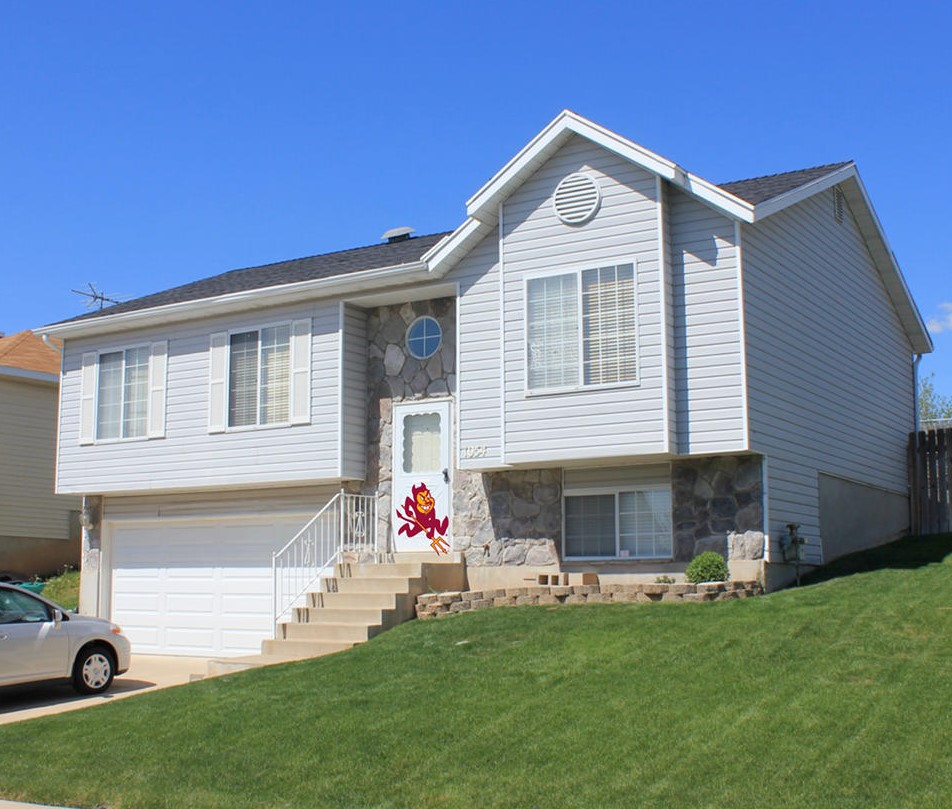
\includegraphics[width=0.7\textwidth]{asu_house.jpg}
        \caption{\tiny{\citeauthor{holton_temporal_2013}\cite{holton_temporal_2013}}}
      \end{figure}
      \begin{itemize}
        \item Near Hill AFB in Layton, UT
        \item TCE contaminated groundwater
        \item Bought by ASU to study VI \& CPM
      \end{itemize}
    \end{column}
    \begin{column}{0.5\textwidth}
      \begin{figure}
        \centering
        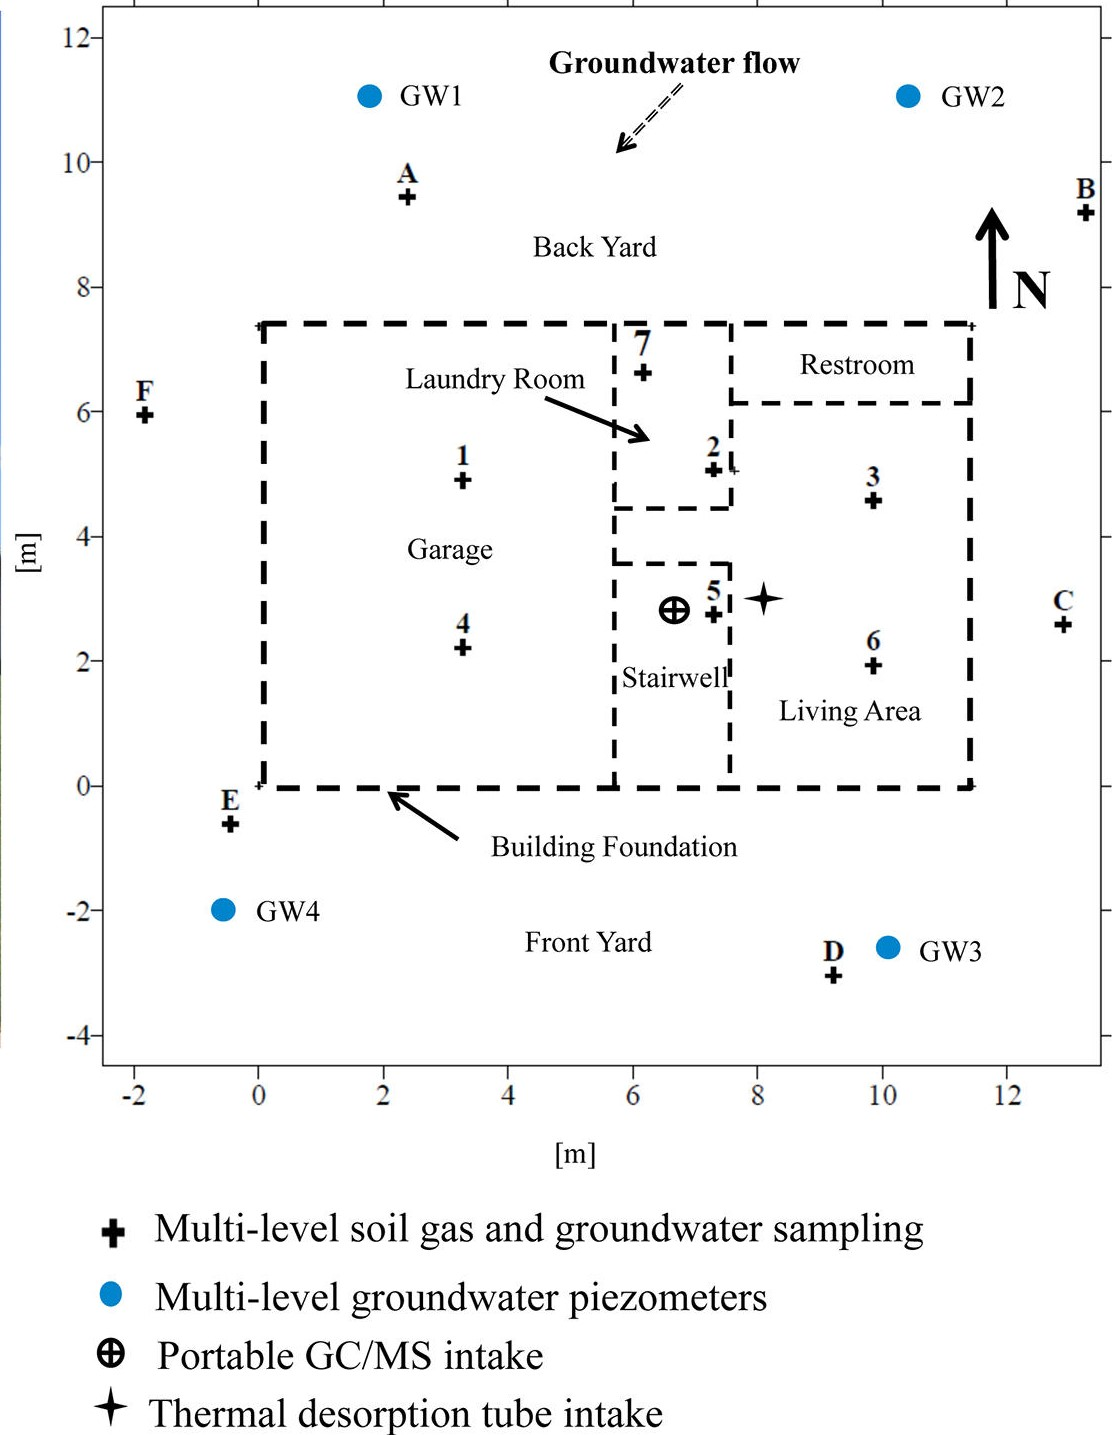
\includegraphics[width=0.9\textwidth]{asu_floorplan.jpg}
        \caption{\tiny{\citeauthor{holton_temporal_2013}\cite{holton_temporal_2013}}}
      \end{figure}
    \end{column}
  \end{columns}
\end{frame}

\begin{frame}
  \frametitle{The Controlled Pressure Method}
  \begin{columns}[T]
    \begin{column}{0.6\textwidth}
      \begin{figure}
        \centering
        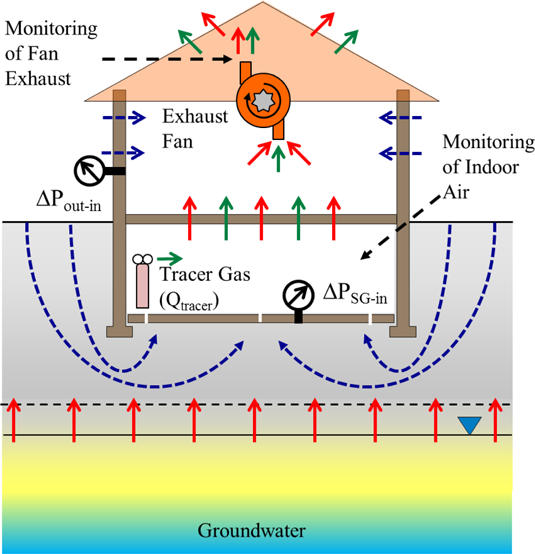
\includegraphics[width=\textwidth]{cpm_cartoon.jpg}
        \caption{\tiny{\citeauthor{holton_long-term_2015}\cite{holton_long-term_2015}}}
      \end{figure}
    \end{column}
    \begin{column}{0.4\textwidth}
      \begin{block}{ }
        \begin{itemize}
          \item Control contaminant entry via building pressurization
          \item Identify indoor sources \& worst-case scenario
        \end{itemize}
      \end{block}
    \end{column}
  \end{columns}

\end{frame}

\begin{frame}
  \frametitle{Discovery of a Preferential Pathway}
    \begin{figure}
      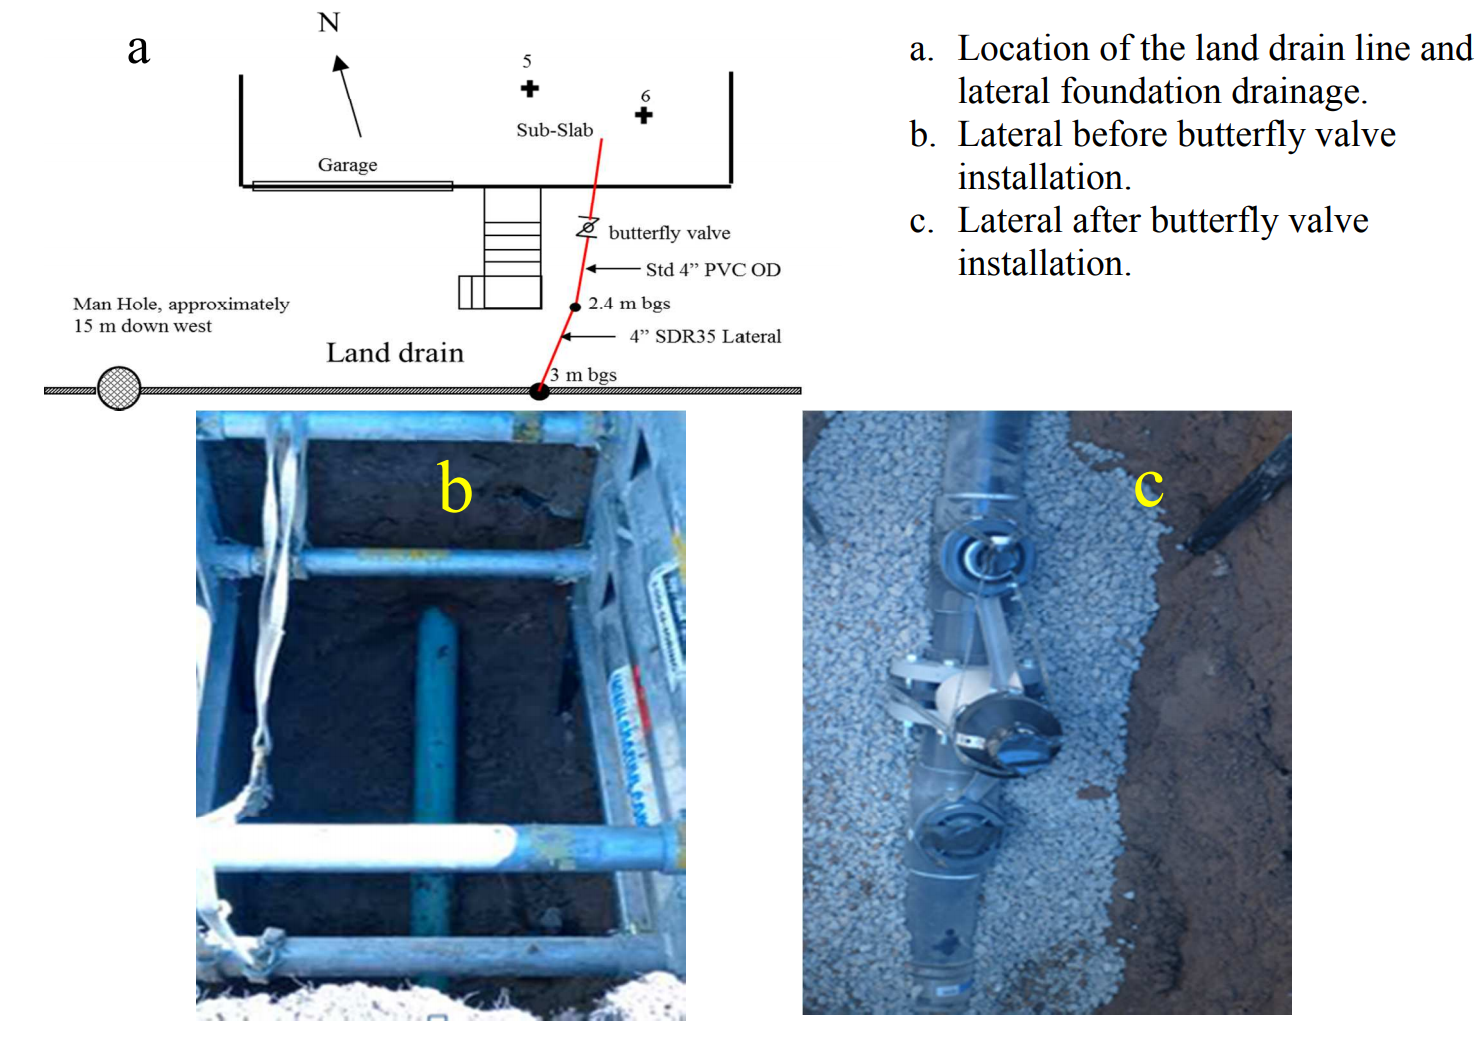
\includegraphics[width=0.8\textwidth]{asu_land_drain.png}
      \caption{\tiny{\citeauthor{guo_identification_2015}\cite{guo_identification_2015}}}
    \end{figure}
\end{frame}

\begin{frame}
  \frametitle{Indoor Contaminant Concentration at the ASU House}
    \begin{figure}
      \centering
      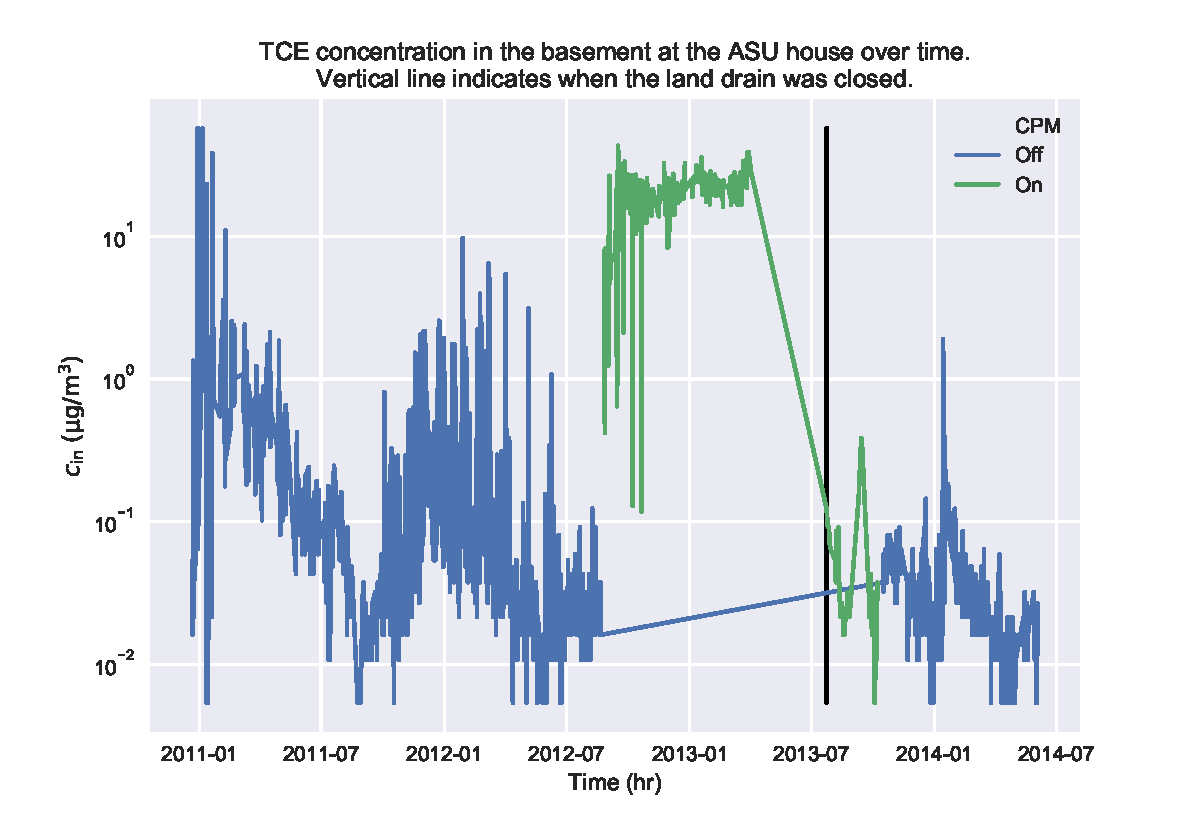
\includegraphics[width=\textwidth]{asu_indoor_concentration.pdf}
    \end{figure}
\end{frame}

\begin{frame}
  \frametitle{Indoor Contaminant Concentration at the ASU House}
    \begin{figure}
      \centering
      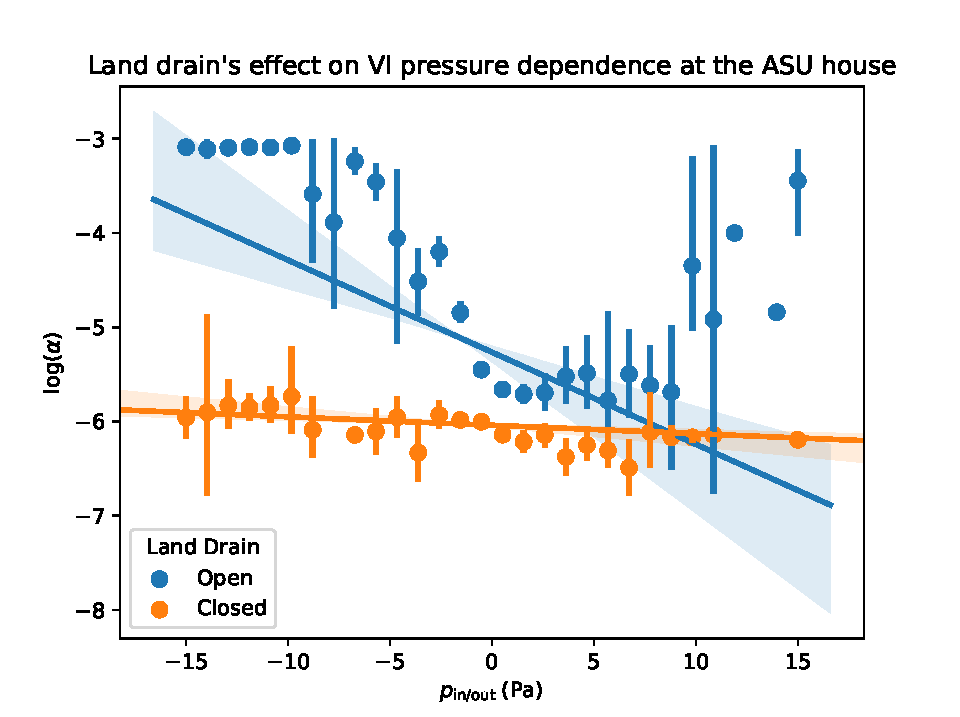
\includegraphics[width=\textwidth]{asu_pressure_dependence.pdf}
    \end{figure}
\end{frame}

% Model description
\begin{frame}
  \frametitle{Modeling a "ASU House"-like VI Scenario}
  \begin{columns}[T]
    \begin{column}{0.6\textwidth}
      \begin{figure}
        \centering
        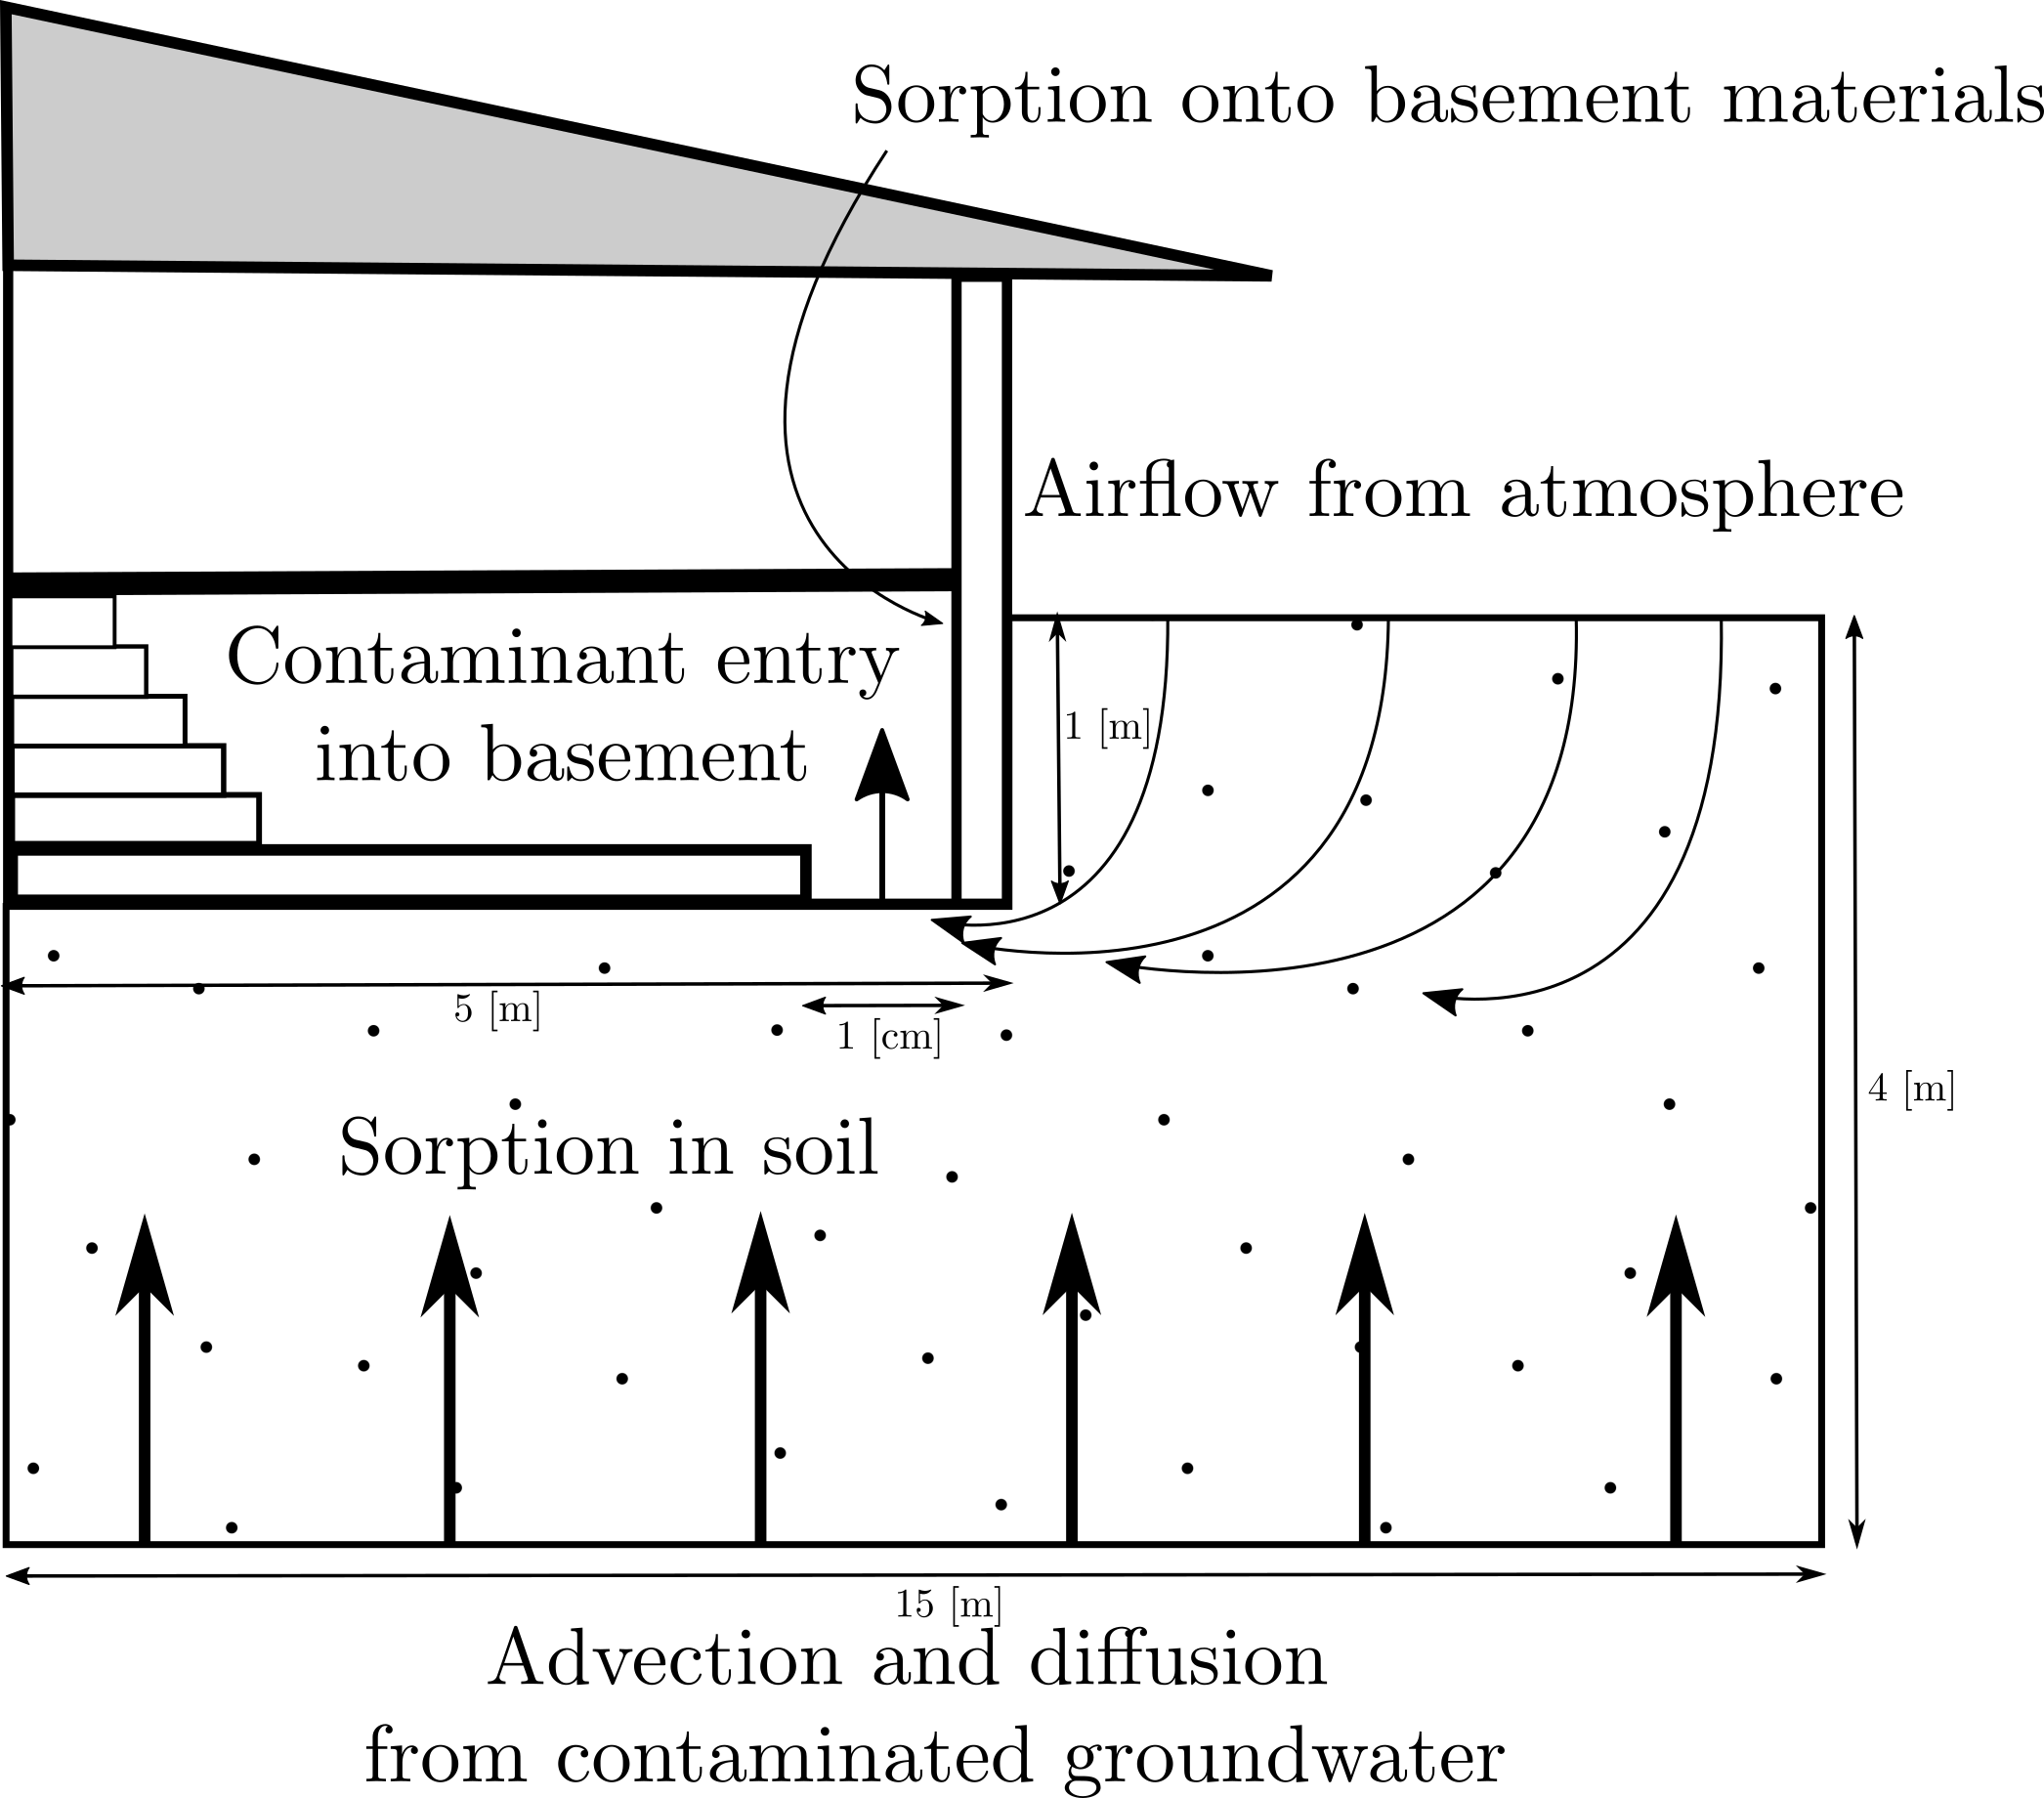
\includegraphics[width=\textwidth]{model.png}
      \end{figure}
    \end{column}
    \begin{column}{0.4\textwidth}
      \begin{block}{Additions}
        \begin{itemize}
          \item Permeable gravel sub-base
          \item 10 cm pipe filled with contaminant vapors
        \end{itemize}
      \end{block}
    \end{column}
  \end{columns}
\end{frame}

% Modeling results
\begin{frame}
  \frametitle{Predicting the Effects of a Preferential Pathway}
  \begin{figure}
    \centering
    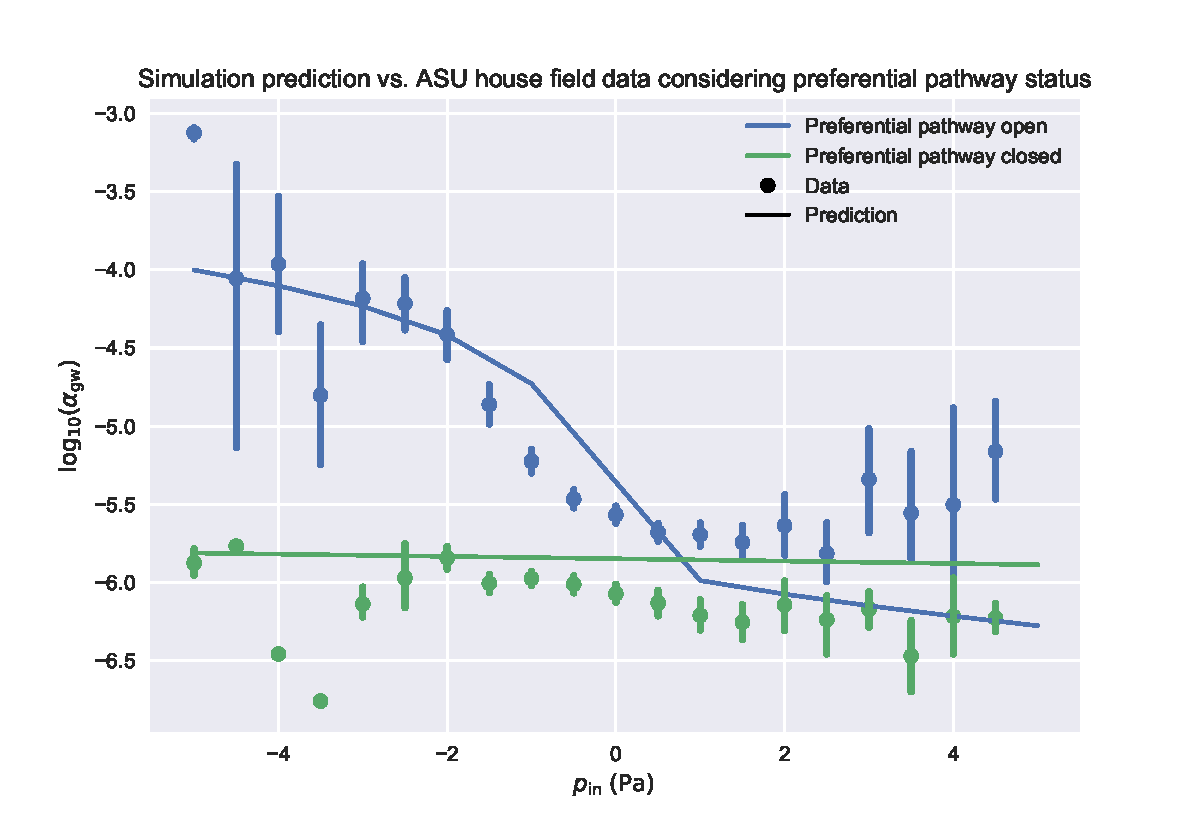
\includegraphics[width=\textwidth]{modeling_results.pdf}
    %\caption{}
  \end{figure}
\end{frame}

% Modeling cases
\begin{frame}
  \frametitle{Preferential pathways: Specific Site Conditions}
  \begin{figure}
    \centering
    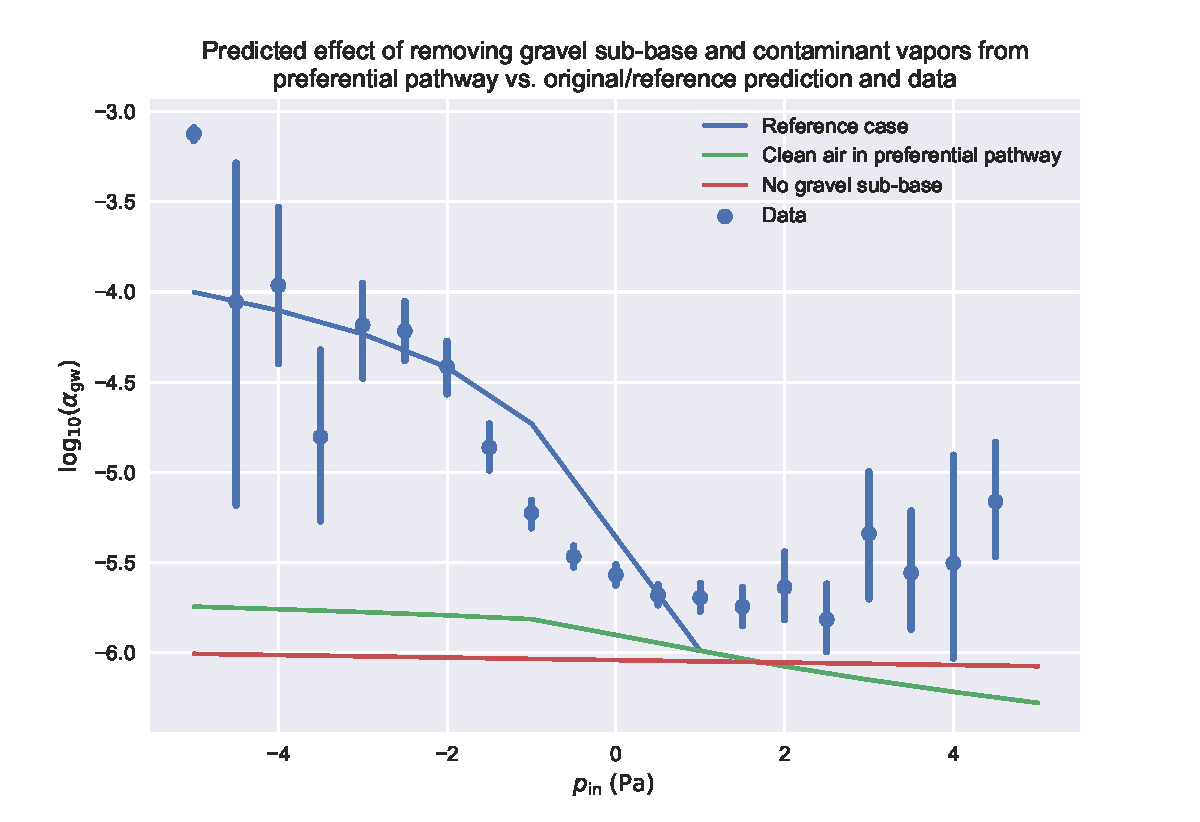
\includegraphics[width=\textwidth]{modeling_cases.pdf}
    %\caption{}
  \end{figure}
\end{frame}

% Peclet number analysis
\begin{frame}
  \frametitle{Péclet Number and Advection}
    \begin{figure}
      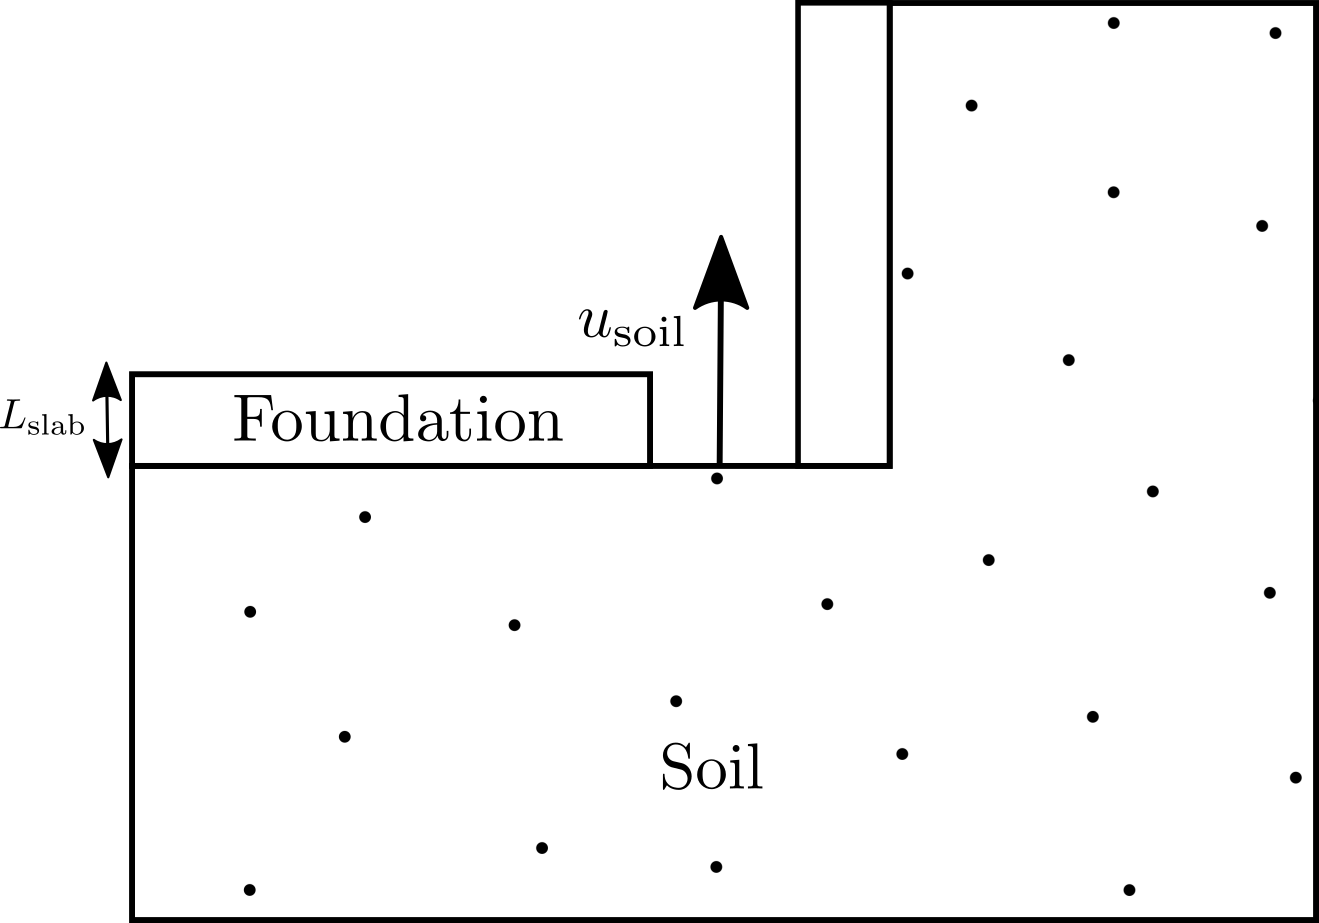
\includegraphics[width=0.5\textwidth]{crack_peclet.png}
    \end{figure}
    \begin{block}{Péclet number for contaminant entry}
      \begin{equation*}
        \mathrm{Pe} = \frac{\mathrm{advection}}{\mathrm{diffusion}} = \frac{u_\mathrm{soil} L_\mathrm{slab}}{D_\mathrm{air}}
      \end{equation*}
      $\mathrm{Pe} > 1 \rightarrow \text{advection dominated}$ \hspace{1em}
      $\mathrm{Pe} < 1 \rightarrow \text{diffusion dominated}$
    \end{block}
\end{frame}

% Peclet number analysis
\begin{frame}
  \frametitle{Péclet Number and Advection}
    \begin{figure}
      \centering
      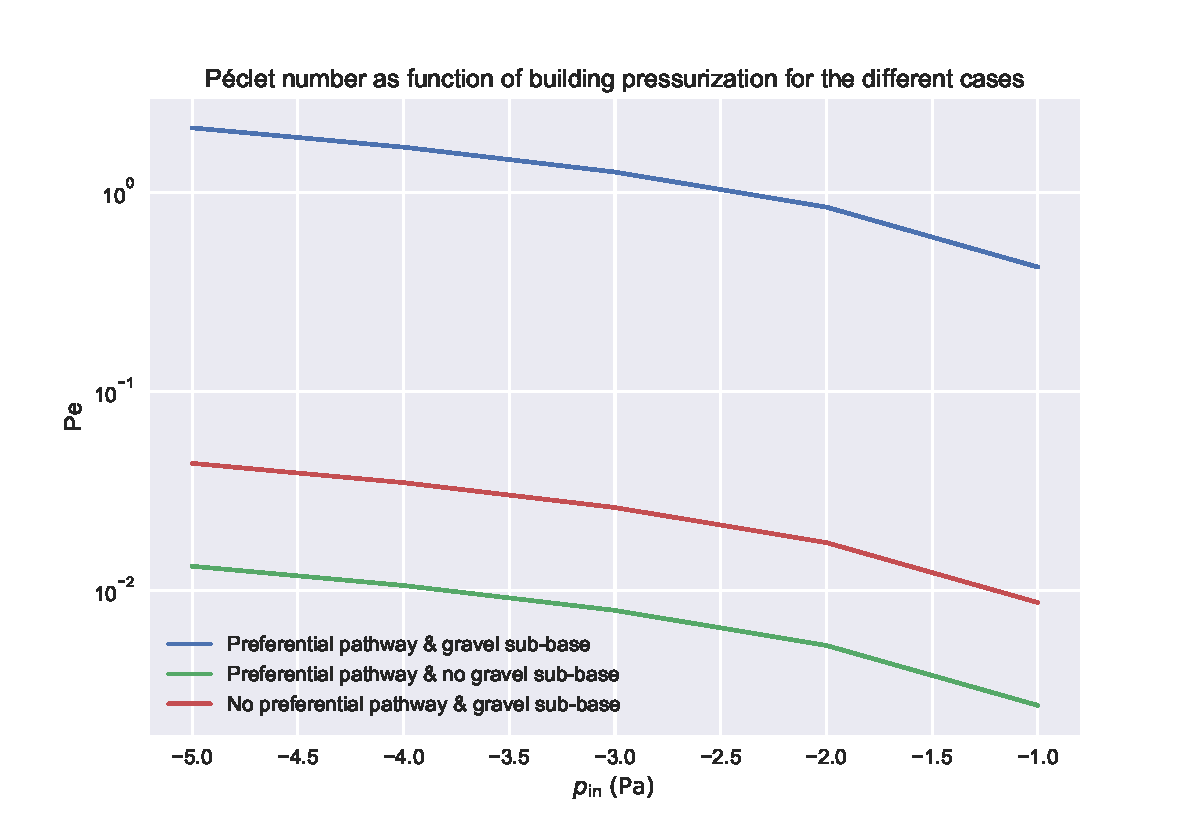
\includegraphics[width=\textwidth]{modeling_result_peclet.pdf}
    \end{figure}
\end{frame}

\begin{frame}
  \frametitle{Advection: Considering Soil and Foundation Type}
    \begin{figure}
      \centering
      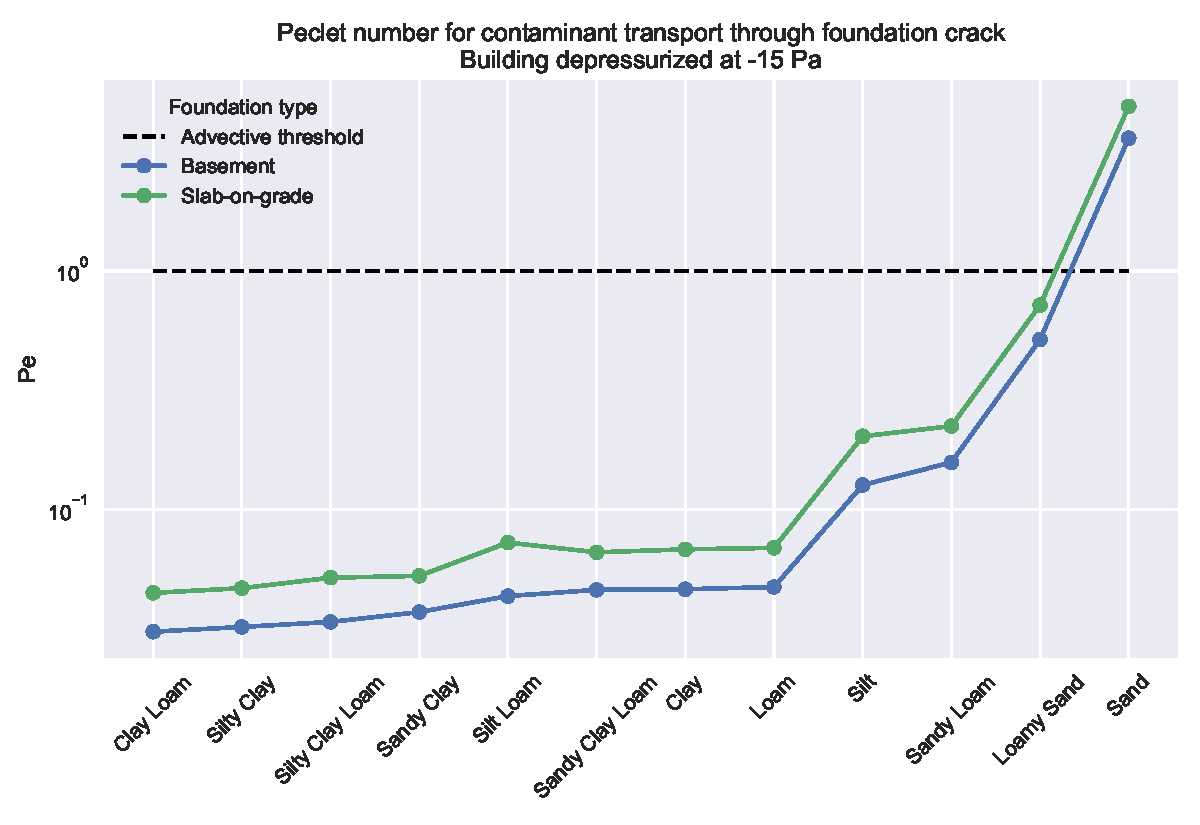
\includegraphics[width=0.8\textwidth]{peclet_cases.pdf}
    \end{figure}
\end{frame}


\begin{frame}
  \begin{alertblock}{Summary}
    \begin{itemize}
      \item Enhanced advective potential explains preferential pathways' significant impact
      \begin{itemize}
        \item Source of air and contaminant
        \item Permeable medium for communication
      \end{itemize}
      \item Challenging assumptions about advective entry - soils unlikely to sustain sufficient flow rates
      \item Insights possible through numerical modeling
    \end{itemize}
  \end{alertblock}
\end{frame}


\begin{comment}
% Including air exchange
\begin{frame}
  \frametitle{Including Air Exchange Rate}
  \begin{figure}
    \centering
    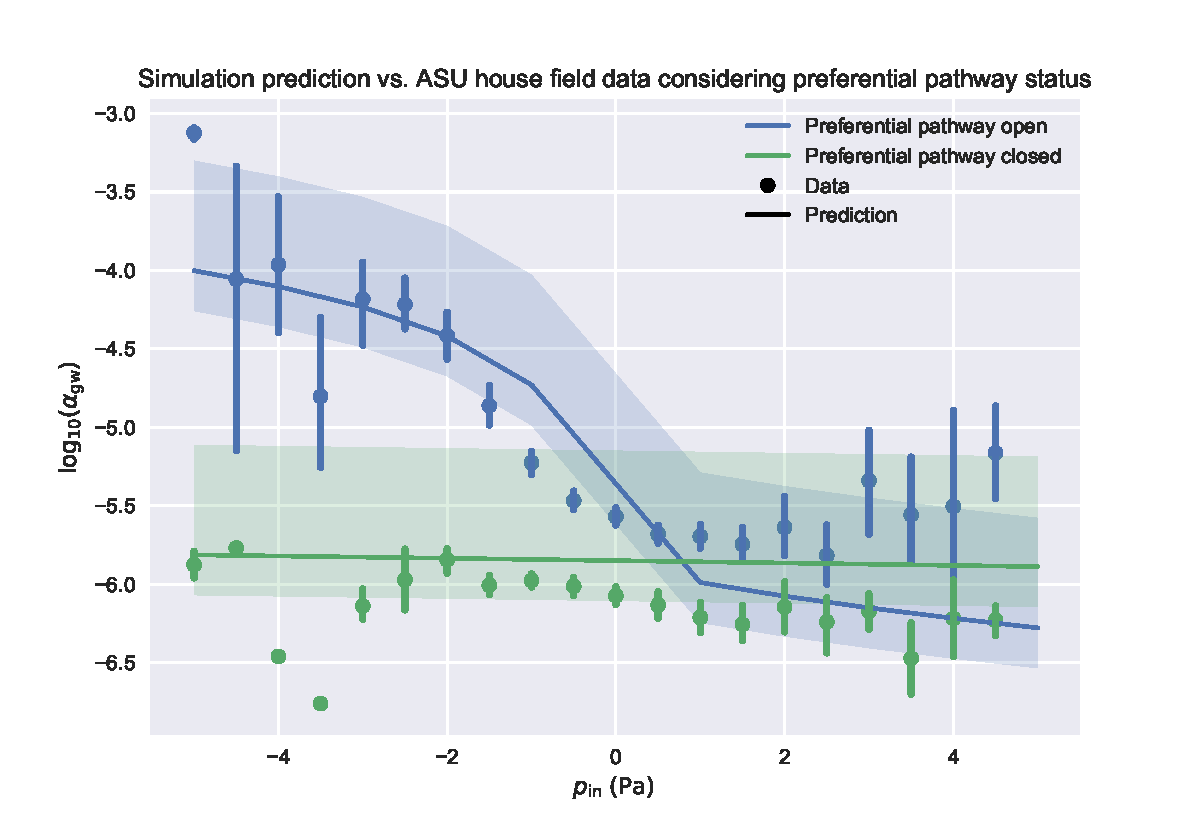
\includegraphics[width=\textwidth]{modeling_result_air_exchange_rate.pdf}
    \caption{}
    \label{}
  \end{figure}
\end{frame}

% Diurnal results
\begin{frame}
  \frametitle{Predicting Daily Variability of Indoor Contaminant Concentration}
  \begin{figure}
    \centering
    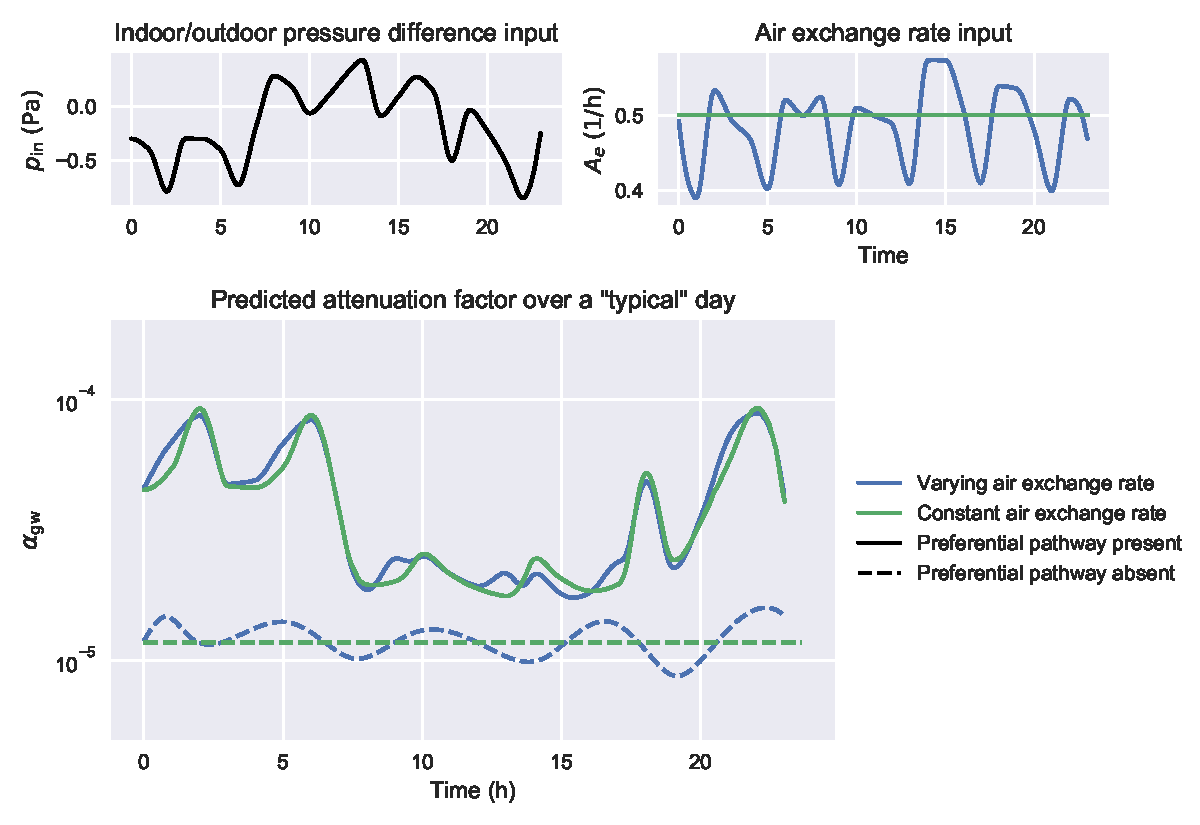
\includegraphics[width=\textwidth]{modeling_diurnal.pdf}
    \caption{}
    \label{}
  \end{figure}
\end{frame}

\end{comment}
